% A Three fold Brochure based on the Latex document class-leaflet
 
\documentclass[notumble,10pt,a4paper]{leaflet} 

% notumble - By default (tumble) the contents of the backside sheet is printed upside down. The option no tumble supresses that.

% Please find the remaining options at http://ctan.math.illinois.edu/macros/latex/contrib/leaflet/leaflet-manual.pdf
\usepackage[utf8x]{inputenc}
\usepackage{fontspec}

\usepackage{color}
\usepackage{flowfram}
\usepackage{graphicx}
\usepackage{wrapfig}
\usepackage{hyperref}      % For including urls
\usepackage{rotating}
\usepackage{multirow}
\usepackage{array}
\usepackage{multirow}
\usepackage{titlesec}
\usepackage[usenames,dvipsnames]{xcolor}
\usepackage{setspace}    % Adjust line spacing    
\onehalfspacing          % Adjust line spacing  \doublespacing 
\usepackage[inline]{enumitem}
%\titleformat*{\subsection}{\color{Blue}}

%FONT Change
%\renewcommand{\familydefault}{cmss} 
%To Draw a horizontal Line
\newcommand{\sectionline}{
  \nointerlineskip \vspace{\baselineskip}
  \hspace{\fill}\rule{0.8\linewidth}{.7pt}\hspace{\fill}
  \par\nointerlineskip \vspace{\baselineskip}
}
%\AddToBackground{2}{\includegraphics[width=29.7cm]{bkf}}
%\AddToBackground{2}{\includegraphics[width=29.7cm]{cmy}}

% To create a border along the top of each page
% To change border color just search on internet for cmyk colour codes and change the values in the brackets after the option cmyk

\vtwotonetop{1cm}{0.6\paperwidth}{[cmyk]{0.35,0,0.67,0.41}}{topleft}%
{0.4\paperwidth}{[cmyk]{0.35,0,0.67,0.41}}{topright}

% To create a border along the bottom of each page
% To change border color just search on internet for cmyk colour codes and change the values in the brackets after the option cmyk

\vtwotonebottom{1cm}{0.6\paperwidth}{[cmyk]{0.35,0,0.67,0.41}}{bottomleft}%
{0.4\paperwidth}{[cmyk]{0.35,0,0.67,0.41}}{bottomright}


\usepackage{listings}
\usepackage{xcolor}
\definecolor{codegreen}{rgb}{0,0.6,0}
\definecolor{codegray}{rgb}{0.5,0.5,0.5}
\definecolor{codepurple}{rgb}{0.58,0,0.82}
\definecolor{backcolour}{rgb}{0.95,0.95,0.92}

\lstdefinestyle{mystyle}{
    backgroundcolor=\color{backcolour},   
    commentstyle=\color{codegreen},
    keywordstyle=\color{magenta},
    numberstyle=\tiny\color{codegray},
    stringstyle=\color{codepurple},
    basicstyle=\ttfamily\footnotesize,
    breakatwhitespace=false,         
    breaklines=true,                 
    captionpos=b,                    
    keepspaces=true,                 
    numbers=none,                    
    numbersep=5pt,                  
    showspaces=false,                
    showstringspaces=false,
    showtabs=false,                  
    tabsize=2
}

\lstset{style=mystyle}


\begin{document}
\begin{center}
	{\Large Arduinio} \\[.3cm]
	%\textit{on}\\[.4cm]
	{\huge {Cheat Sheet}}\\ [.3cm]
	
	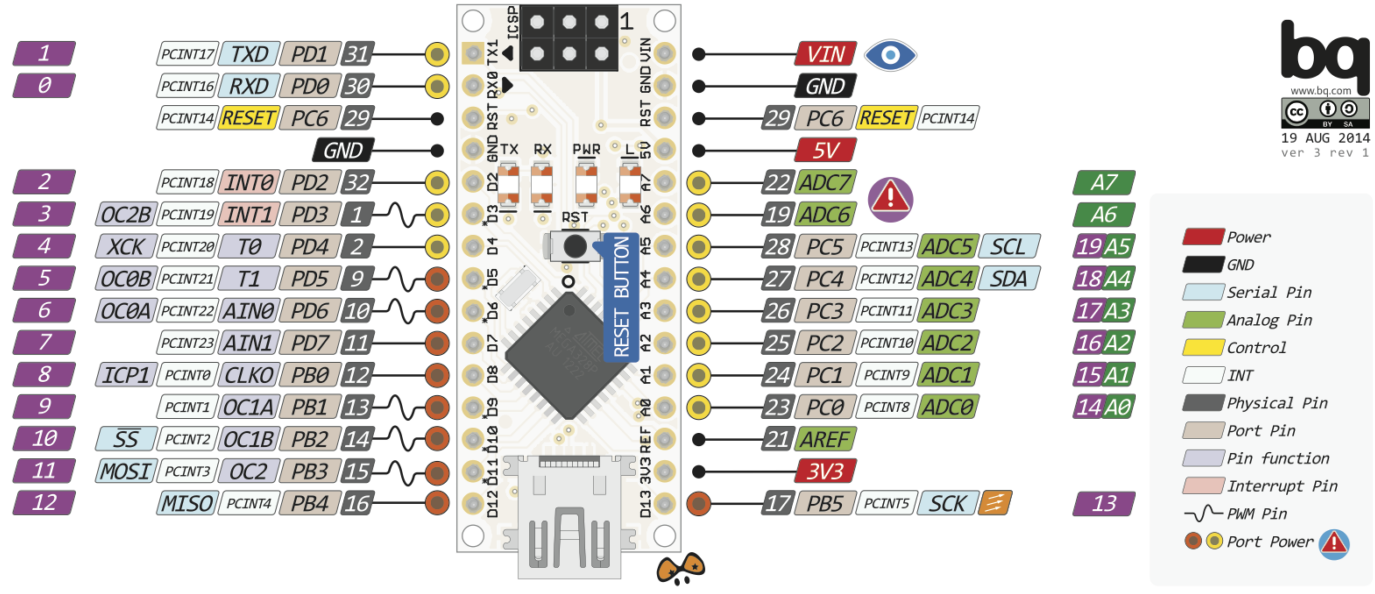
\includegraphics[width=\linewidth]{pictures/nanoFull.png}\\
	\label{fig:Pinout}

	
	\vfill
	created by\\ 
	\textbf{WAK-Lab e.V. Eisenach}\\
	Web:\url{https://wak-lab.org}
\end{center}


\thispagestyle{empty} 
\newpage
\subsection{\large{Arduino IDE}}
Die Arduino IDE ist eine Programmierumgebung für C++ ohne den Nutzer gleich mit zu vielen Konwentionen zu überlasten wird der Quelltext in einer einzigen ,,ino`` Datei im geichnamingen Verzeichnis gepeichert. Nichts desdo trotz sind im Hitergrund umfangreiche Bibliotheken für Hardware- und Softwaremodule versteck. In der Werkzeugliste findet man dafür den Biblioteks und den Bordverwalter. Außerdem können in den Voreinstellungen auch externe Quellen eingebunden werden.\\
\subsection{\large{Programmstruktur}}
Das Programm besteht im wesentlichen aus einer \textit{setup()} Fuktion die beim Start aufgerufen wird und eine \textit{loop()} Schleife die auch wenn sie beendet ist immer wieder vom Prozessor aufgerufen wird.\\
\begin{lstlisting}[language=c, caption=Beispiel]
// Ganzzahl (integer) im Bereich von -32768 bis 32767 
int EineGlobaleVariable; 
void setup() {
  // Dieser Code wird beim Start aufgerufn
  // Diese Variable existiert nur so Lange Setup läuft
  int EineLokalVariable;  
}

void loop() {
  // Dieser Code wird immer wieder aufgerufen
  // Diese Variable existiert dauerhaft und behält ihren Wert beginnend mit 0
  static int EineLokalStatischeVariable = 0; 
}
\end{lstlisting}
\newpage
\subsection{\large{Bibliotheken verwenden}}
Bibliotheken sind Voreinstellung und Bauanleitungen für Funktionalitäten die wir einfach benutzen wollen ohne uns groß in Details zu verstricken. Die wichtigsten Bibliotheken sind bereits automatisch eingebunden ohne dass wir davon etwas in der Arduino IDE mitbekommen.
\subsection{Serial}
Die Verbindung zum seriellen Monitor ermöglicht uns, dass das Board Texte und Zahlen an die Oberfläche senden kann. Damit können wir lesen, was der Prozessor gerade mancht. 
\begin{lstlisting}[language=c, caption=Beispiel]
void setup() {
  Serial.begin(9600);
}

void loop() {
  Serial.println("Hallo World");
  // Eine Wartezeit von 1000 Millisekunden wartet 1 Sekunde    
  delay(1000);        
}
\end{lstlisting}


\subsection{\large{Eingänge}}
\begin{lstlisting}[language=c, caption=Beispiel]
void setup() {
   // Pin 2 als Eingang definieren
  pinMode(2, INPUT); 
}
void loop() {
  // Digitaler Eingang 2 einlesen
  int buttonState = digitalRead(2); // 
  // Analogen Eingang A0 einlesen
  int sensorValue = analogRead(A0); 
\end{lstlisting}

\subsection{\large{Ausgänge}}

\newpage
\subsection{\large{Strings}}

Text

\begin{itemize*} %use itemize without the asterik to get the usual list appearance
	\item Test
\end{itemize*}

\subsection{\large{Section 2}}
\noindent
\begin{tabular}{@{}ll}
	Tabelle & Datum\\
	Eintrag    & Info\\
\end{tabular}

{\large\textbf{{Contact}}}\\
\url{info@wak-lab.org}

\begin{center}
\textbf{Apply} \\
Hier könnte ihr QR-Code stehen\\
%\begin{figure}[h!]
%	\centering
%	\includegraphics[width=0.3\linewidth]{QR-Code}
%\end{figure}
\end{center}

\newpage

\section{\large{Section 3}}


\subsection{\large{Contact}}
WAK-Lab.e.v\\
CNebestraße 24\\
99817 Eisenach\\
Germany\\
Email:  \url{info@wak-lab.org}

\newpage
\vspace*{\fill}
\begin{center}
%	\begin{figure}[h!]
%		\centering
%		\includegraphics[width=0.3\linewidth]{Kontakt bild}
%	\end{figure}
%	\Large{\textbf{\url{https://wak-lab.org}}}	
\end{center}
\vspace*{\fill}


\end{document}
